\section{Subsistema: Mecânica e Alimentação}

  \subsection{Sistema de Tração}

  Para a análise comparativa foram estudadas e consideradas as características dos principais tipo de sistemas de tração,
  afim de escolher um sistema que atenderá todas as necessidades do projeto sendo o menos oneroso.

  \begin{itemize}
    \item Sistema de Esteira

    O sistema de tração por esteiras é largamente utilizado em aplicações agrícolas e em aplicações gerais nas quais é necessária
    a locomoção em terreno acidentado. O sistema tradicional de transmissão mecânica por esteiras é formado por diversos componentes,
    como conversor de torque, amortecedores e \textit{dumpers}.
    Este sistema possui como vantagem o alto fornecimento de tração ao veículo, mas requer um grande espaço para acoplamento ao mesmo,
    além da baixa disponibilidade de materiais para sua fabricação. Outra desvantagem é que este sistema impede que o veículo realize
    manobras de contra-rotação.

    \item Sistema de Rodas

    O sistema de rodas consiste na configuração mais utilizada em todos os tipos de veículos, a literatura é bastante consolidada
    no que se refere a sistemas de transmissão e acoplamentos para veículos movidos sobre rodas. Este sistema foi o escolhido para
    implantação neste projeto devido à sua viabilidade de projeto e fabricação.
    Foi realizada uma pesquisa de modelos de rodas disponíveis, tendo como requisito um diâmetro de aproximadamente 10cm e pneus com
    perfil off-road, conforme mostra a figura \ref{WHEELS}.

    \begin{figure}[!htb]
    \begin{center}
    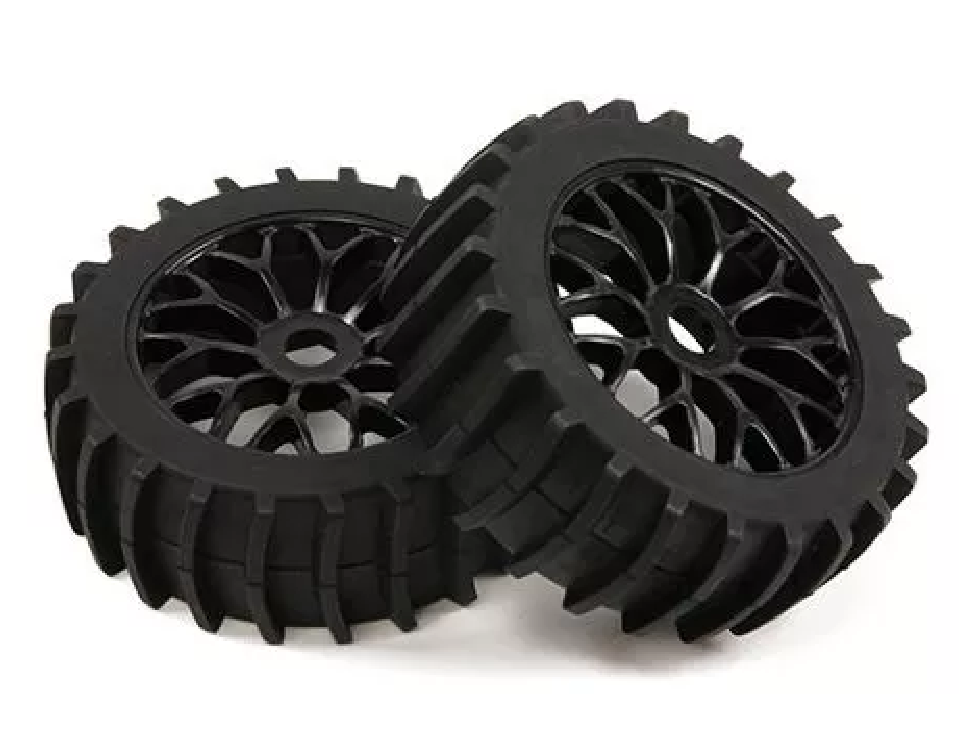
\includegraphics[keepaspectratio=true,scale=0.3]{figuras/wheels.eps}
    \caption{\label{WHEELS}Modelo de rodas}
    \end{center}
    \end{figure}

		\newpage
    \item Sistema Aranha

    Este sistema de locomoção é bastante engenhoso. Consiste em vários braços, geralmente 6 ou 8, comandados por 2 motores ou
    mais em cada braço. Este sistema pode ser usado nos mais diversos tipos de terreno por fornecer alta estabilidade e tração
    satisfatória. A cinemática envolvida na movimentação e no controle deste tipo de sistema é muito mais complexa do que nos
    sistemas de locomoção por esteira e por rodas, devido ao alto número de motores requeridos.

  \end{itemize}

  Dentre as outras alternativas, adotou-se a locomoção baseada em rodas, pois são mais comumente encontrados na robótica móvel,
  tendo em vista o baixo custo, seja na implementação como na manutenção, fornece uma boa estabilidade, além de sua simplicidade
  mecânica. Como será aplicado em terrenos planos com algumas irregularidades, sem grandes declives e aclives \cite{matsumura2014desenvolvimento}, portanto a alternativa
  atende bem a proposta.

  Foi escolhido rodas de diâmetro grande, pois com ela o sistema de tração
  fica mais simples e com custos menores. O veículo também poderá passar por
  pequenos obstáculos sem dificuldades. Com esse conjunto o robô ficará elevado
  em relação ao solo, levando em conta seu centro de gravidade e demais
  componentes atuando. A figura~\ref{WHEEL} mostra o tipo de roda relatada.

  \begin{figure}[!htbp]
  \begin{center}
  \includegraphics[keepaspectratio=true,scale=0.5]{figuras/wheel2.eps}
  \caption{\label{WHEEL}Roda escolhida para o projeto.}
  \end{center}
  \end{figure}

  \newpage
  \vfill
  \pagebreak

  \subsection{Sistema de Direção}
    O sistema de direção é composto por um conjunto de barras em forma de garfo, 
    que são movidas por um motor de passo modelo 22KM–0213G6V. Este motor tem seu torque aumentado através de um par de engrenagens, cuja relação é de 5 pra 1. O eixo atravessa uma das barras do chassi e utiliza uma bucha e dois rolamentos para permitir a livre rotação eixo de direção.  
     
    A escolha do motor de passo é motivada pela capacidade de posicionamento angular, que é realizado pelo movimento de passos do motor, e possui a relação de 1,8$^o$ por passo, além de seu torque. O seu posicionamento angular é transmitido para a roda, fazendo com que a mesma possa realizar curvas durante o trajeto e manter a distância correta da fileira a ser perfurada. 
    
    O motor de passo será conectado a barra por meio de um acoplamento, que transmitirá todo o movimento à roda. O layout da estrutura do sistema de direção é mostrado abaixo. 
    
    
    \begin{figure}[!htbp]
                    	\begin{center}
                    		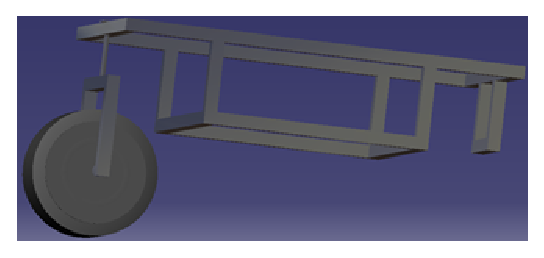
\includegraphics[keepaspectratio=true,scale=1]{figuras/direcao1.eps}
                    		\caption{Sistema de direção acoplado ao chassi}
                    	\end{center}
     \end{figure}
                    
     \begin{figure}[!htbp]
                    	\begin{center}
                    		(a)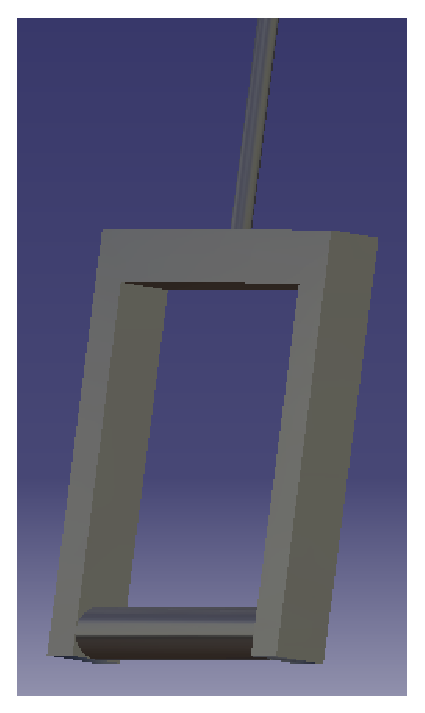
\includegraphics[height=.3\textheight]{figuras/direcao2.eps}
                    		(b)\includegraphics[height=.3\textheight]{figuras/motor_passo.eps}
                    		\caption{(a) Garfo a ser conectado a roda e ao motor de passo; (b) Motor de passo com par de engrenagens.}
                    	\end{center}
      \end{figure}
    
    Para o controle de direção do veículo foi escolhido um motor de passo bipolar \cite{brites}. Estes são dispositivos eletromecânicos que convertem pulsos elétricos em movimentos mecânicos que geram variações angulares discretas. O rotor ou eixo de um motor de passo é rotacionado em pequenos incrementos angulares, denominados “passos”, quando pulsos elétricos são aplicados em uma determinada sequência em seus terminais. A rotação de tais motores é diretamente relacionada aos impulsos elétricos que são recebidos, bem como a sequência a qual tais pulsos são aplicados reflete diretamente na direção a qual o motor gira.
    
        \begin{figure}[h]
        	\centering
        	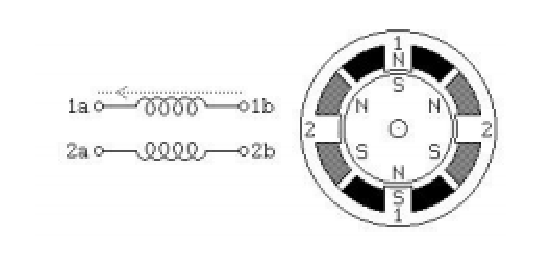
\includegraphics[keepaspectratio=true, scale=1]{figuras/passo_unipolar.eps}
        	\caption{Motor de passo unipolar}
        	\label{fig:unipolar}
        \end{figure}
    
    Conforme ilusta a Figura \ref{fig:unipolar}, o funcionamento básico do motor de passo é dado pelo uso de solenoides alinhados dois a dois que quando energizados atraem o rotor fazendo-o se alinhar com o eixo determinado pelos solenoides, causando assim uma pequena variação de ângulo, chamada de passo. A velocidade e o sentido de movimento são determinados pela forma como cada solenoide é ativado. Os motores bipolares têm um único enrolamento por fase. A corrente em um enrolamento precisa ser invertida a fim de inverter um polo magnético, assim o circuito de condução é um pouco mais complicado, e necessita de um arranjo de ponte H \cite{brites}.
    
    Ponte H é um circuito eletrônico que permite que um motor rode tanto para um sentido quanto para o outro. O nome ponte H é dado pela forma que assume o circuito quando montado. O circuito é construído com quatro “chaves” que são acionadas de forma alternada. Para cada configuração das chaves o motor gira em um sentido.
    
    Considerando as necessidades inerentes ao sistema de direção, buscou-se um modelo capaz de prover robustez, alto torque e viabilidade de controle. Sendo assim foi escolhido um NEMA 23 da Matsushita, que apresenta uma tensão de operação na faixa de 12 a 36V e um torque de até 10kgf.cm. Além disso, sua resolução de passo é de 1.8$^o$, e sua corrente de entrada máxima é de 2A. Para o seu controle, foi utilizada a biblioteca “accelstepper” disponibilizada pela Adafruit. Vale ressaltar que o motor será acoplado a uma caixa de redução, logo o torque resultante na direção será superior ao fornecido pelo motor. 
    
            \begin{figure}[h]
            	\centering
            	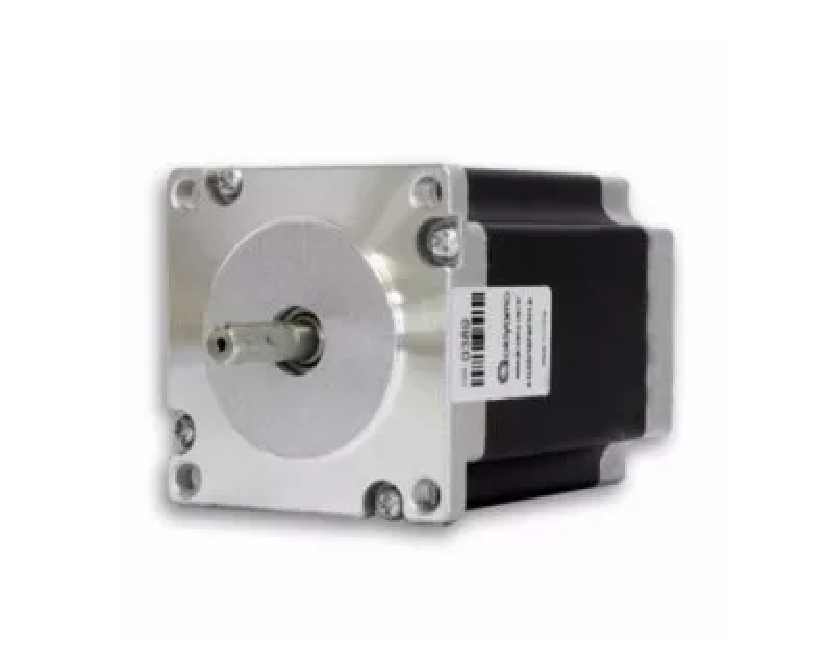
\includegraphics[keepaspectratio=true, scale=1]{figuras/matsu.eps}
            	\caption{Matsushita NEMA 23. Fonte: \cite{bde}}
            	\label{fig:matsu}
            \end{figure}
    
    Tendo em vista a necessidade de utilização de uma ponte H, foram considerados diversos circuitos desenvolvidos especificamente para o controle de motores. Dentre as opções disponíveis, escolheu-se o A4988 fabricado pela Allegro. Este circuito, ilustrado na Figura \ref{fig:drivepasso}, é um \textit{driver} de micro-passo completo desenvolvido para fácil operação. Além disso, ele foi projetado para operar motores de passo bipolares em diversas configurações de passo e apresenta uma capacidade de condução de saída de até 35 V e aproximadamente 2 A.
    
                \begin{figure}[!h]
                	\centering
                	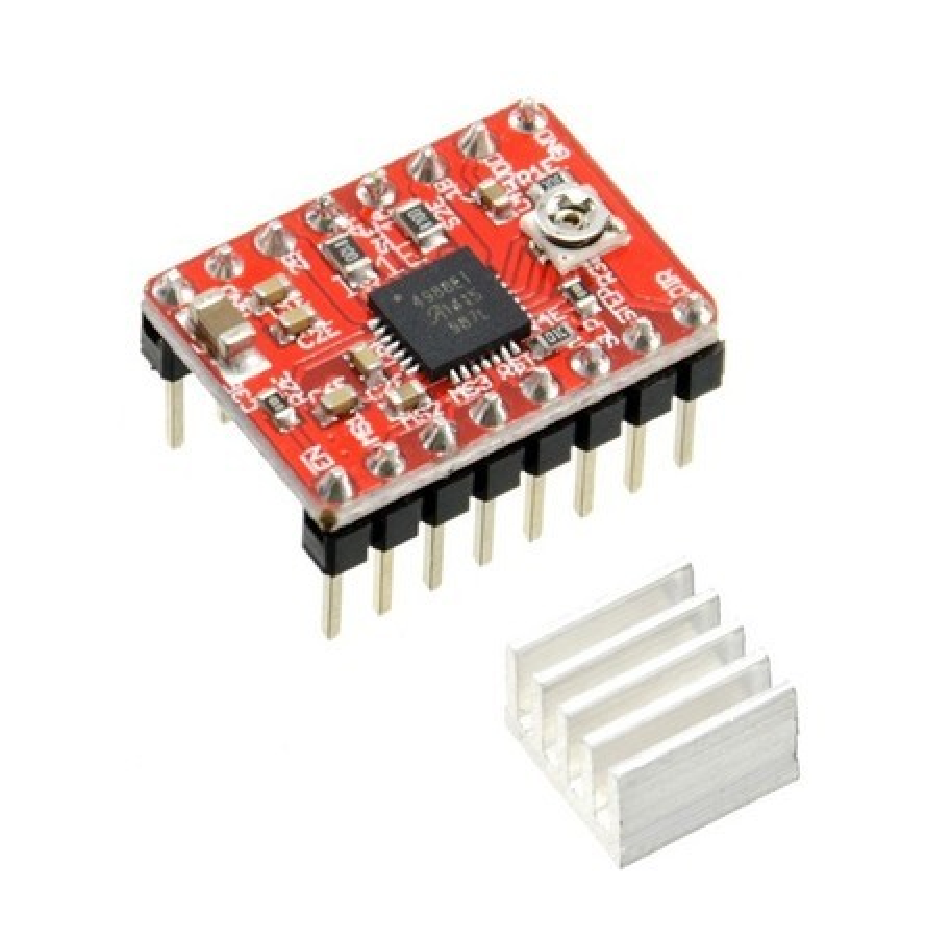
\includegraphics[keepaspectratio=true, scale=0.4]{figuras/drive_passo.eps}
                	\caption{Driver Allegro A4988. Fonte: \cite{flop}}
                	\label{fig:drivepasso}
                \end{figure}
                

      
  \subsection{Estrutura}
  Após a definição dos sistemas que compõem a parte mecânica deste projeto é necessário a definição de uma estrutura externa para o veículo (rodas, pneus, chassi, eixos e carenagem). Foi feita uma pesquisa para verificar quais materiais atenderiam as necessidades da estrutura do veículo. Portanto seguem as tabelas comparativas de possíveis materiais a serem usados.

  \begin{table}[!htbp]
  \begin{center}
  \caption{Roda e Pneu}
  \begin{tabular}{|p{2cm}|p{3cm}|p{2cm}|}
  \hline
  \textbf{Roda e Pneu} & \textbf{Descrição} & \textbf{Imagem}\\\hline\hline
  Tipo 1 & Roda de MBS Atom, 80/85 ou Colt 80 placas, de 7 polegadas & 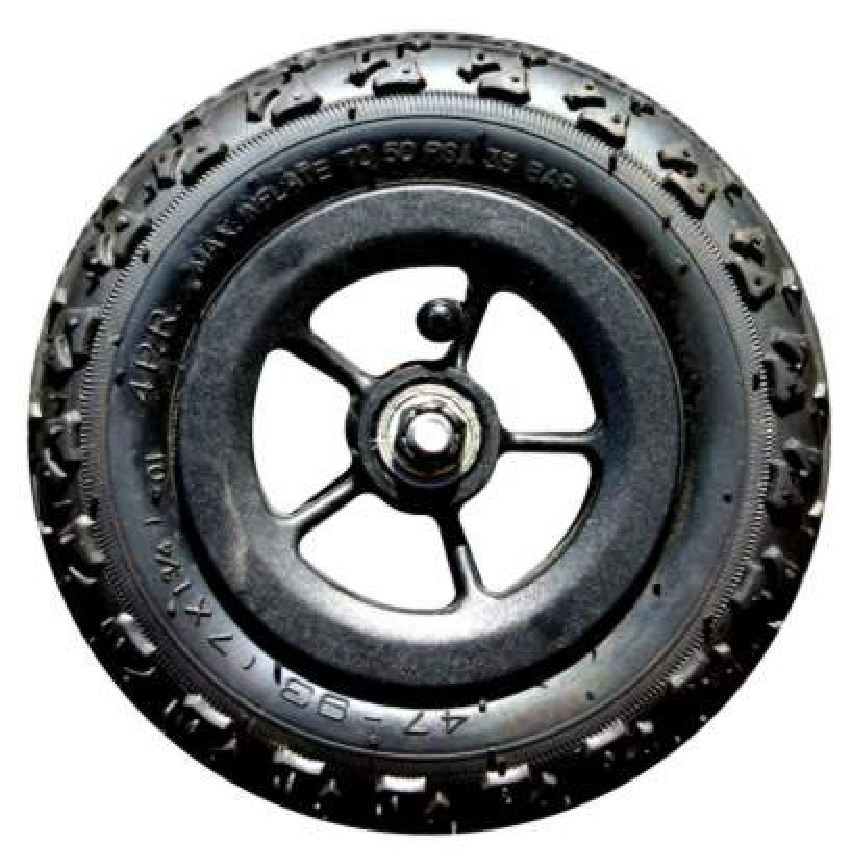
\includegraphics[width=2cm]{figuras/roda_mbs.eps}\\\hline
  Tipo 2 & Rodas 17mm Buggy Off Road Pneu Para Areia E Terra -FH & 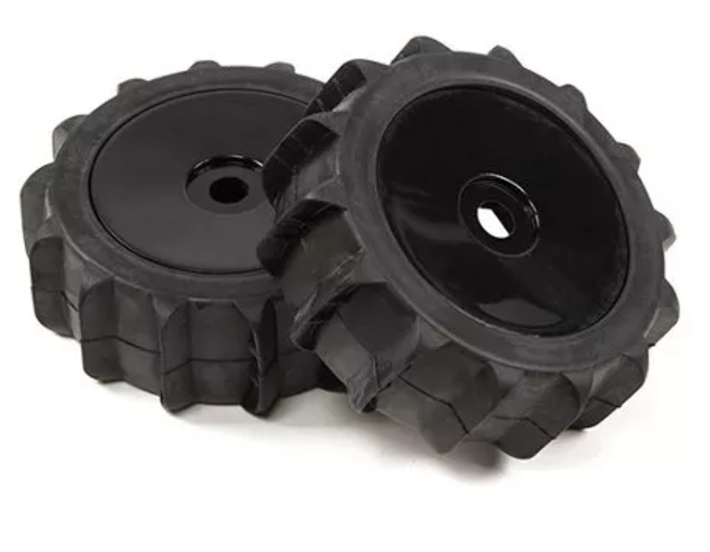
\includegraphics[width=2cm]{figuras/roda_buggy.eps}\\\hline
  \end{tabular}
  \end{center}
  \end{table}

  \begin{table}[!htbp]
  \begin{center}
  \caption{Chassi}
  \begin{tabular}{|p{2cm}|p{3cm}|p{2cm}|}
  \hline
  \textbf{Chassi} & \textbf{Material} & \textbf{Imagem}\\\hline\hline
  Tipo 1 & Aço inox & 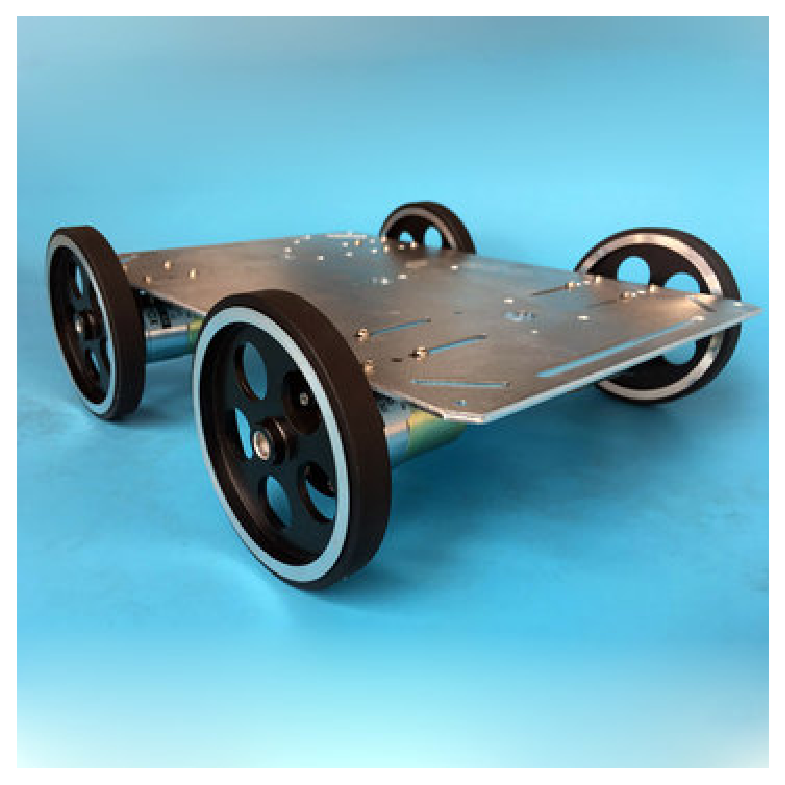
\includegraphics[width=2cm]{figuras/chassi_inox.eps}\\\hline
  Tipo 2 & Aluminio & 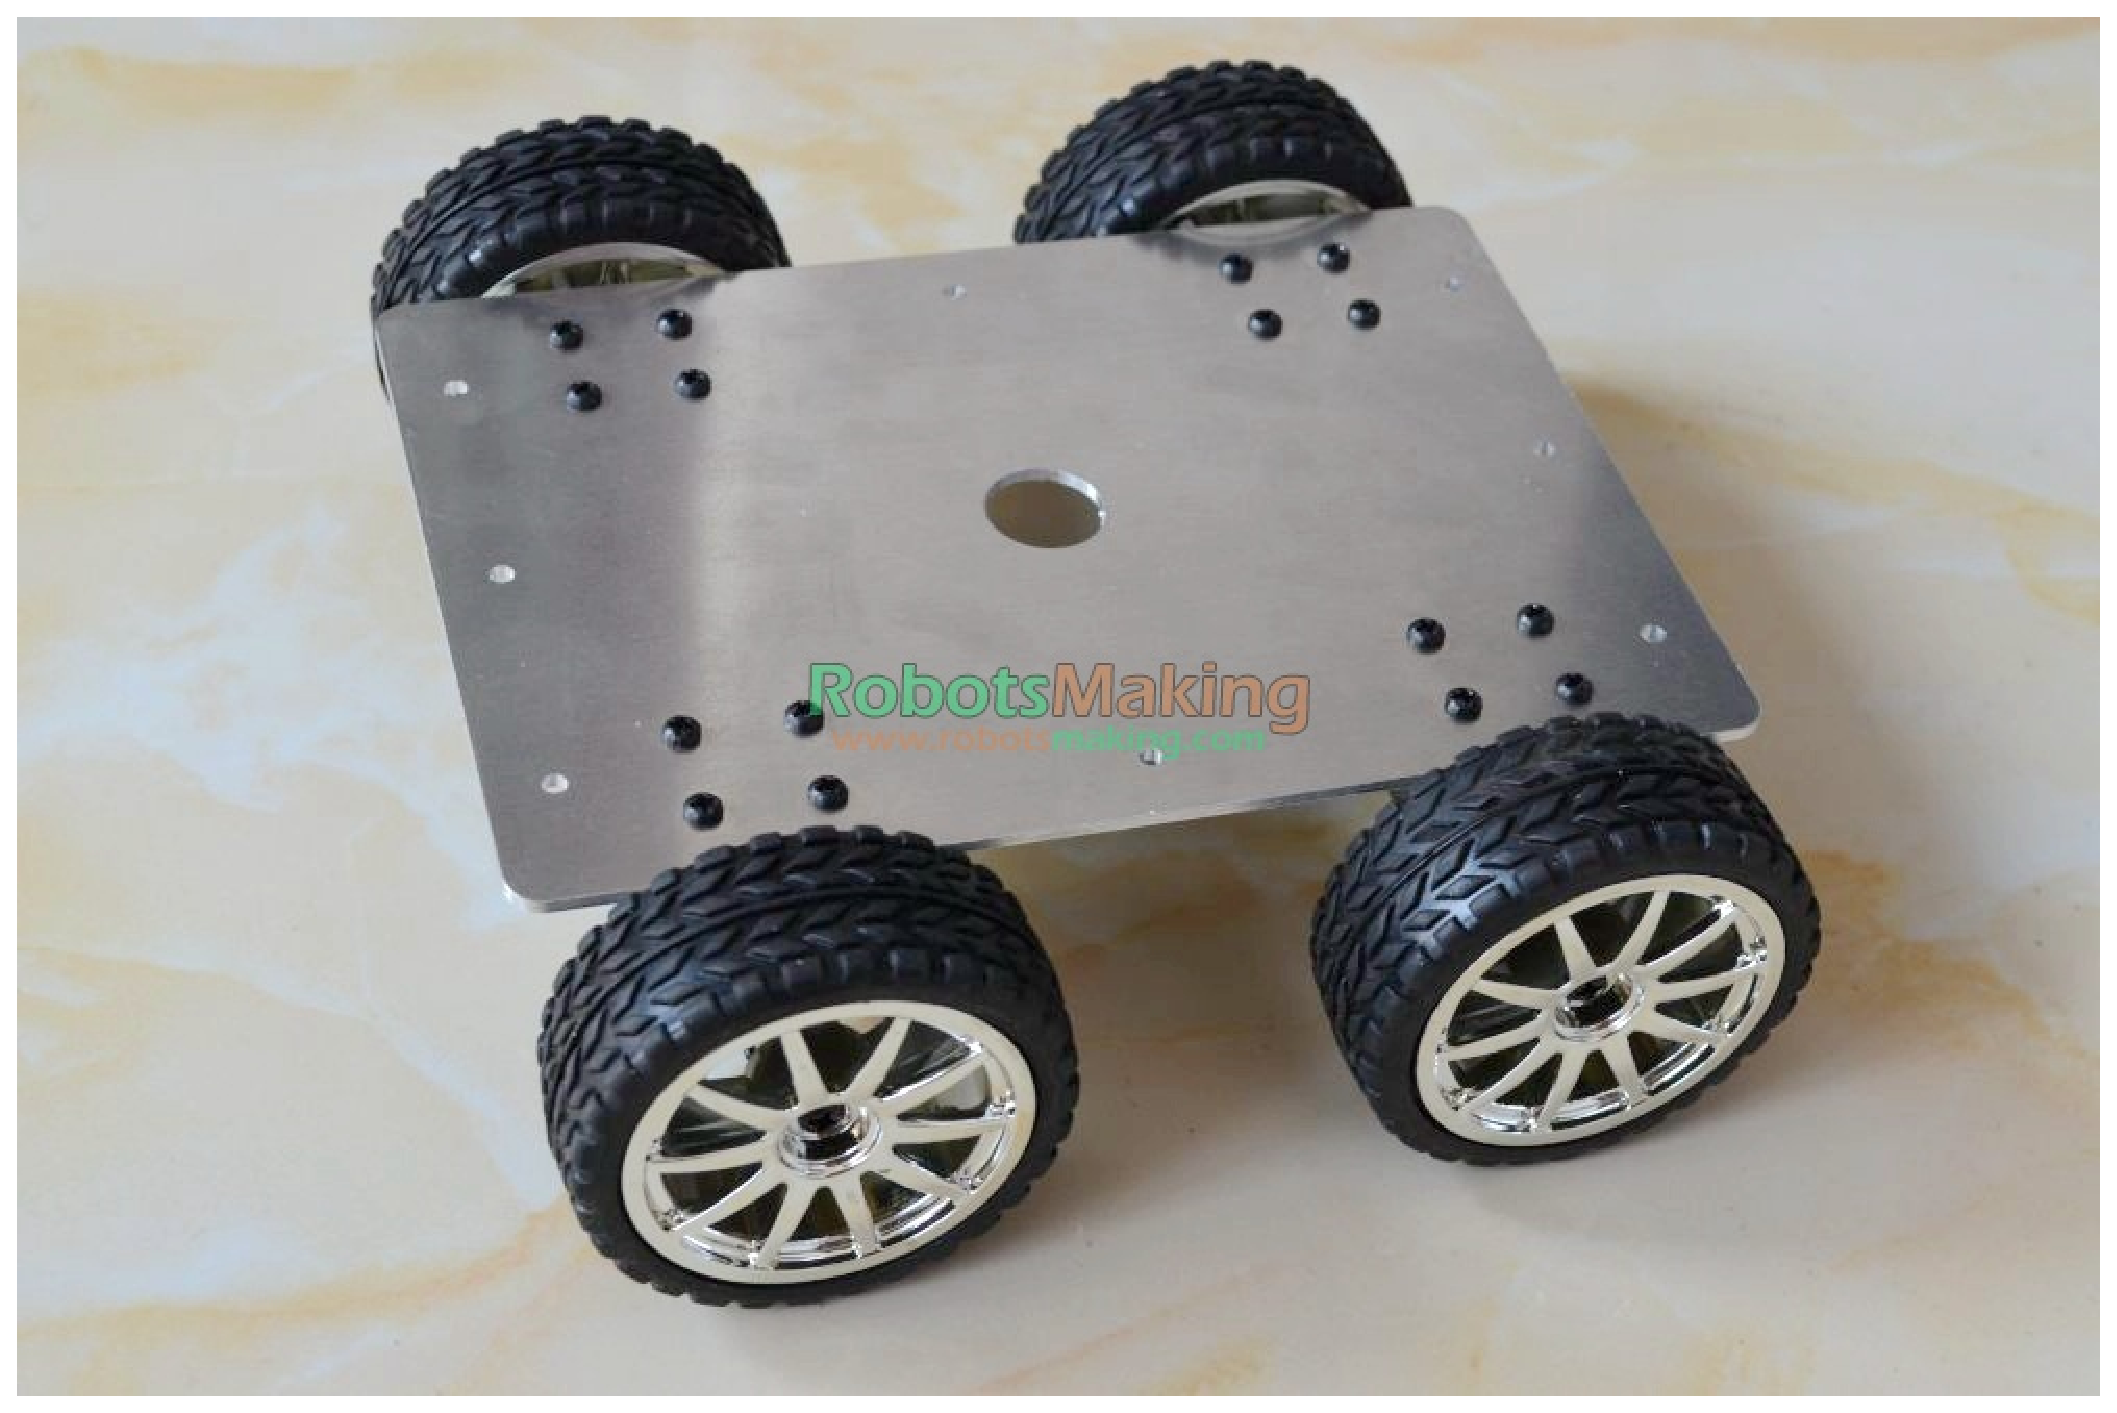
\includegraphics[width=2cm]{figuras/chassi_aluminio.eps}\\\hline
  \end{tabular}
  \end{center}
  \end{table}

  \begin{table}[!htbp]
  \begin{center}
  \caption{Eixo}
  \begin{tabular}{|p{2cm}|p{3cm}|p{2cm}|}
  \hline
  \textbf{Eixo} & \textbf{Material} & \textbf{Imagem}\\\hline\hline
  Tipo 1 & Aço inox & 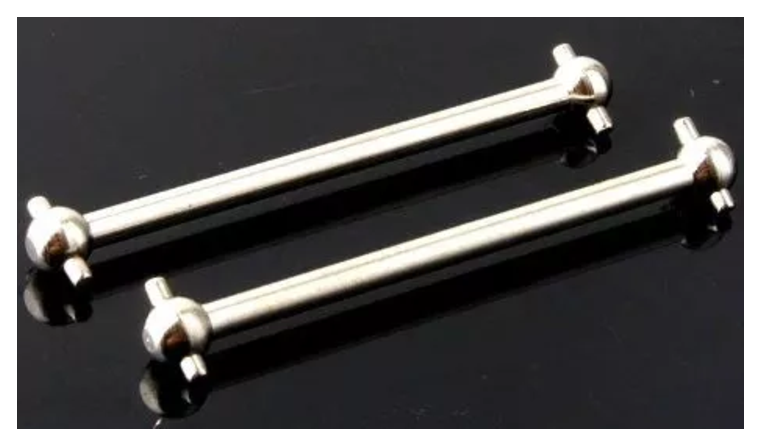
\includegraphics[width=2cm]{figuras/eixo_inox.eps}\\\hline
  Tipo 2 & Aluminio  & 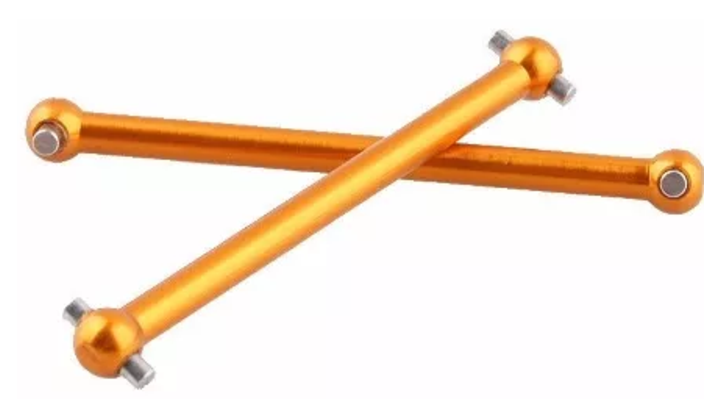
\includegraphics[width=2cm]{figuras/eixo_aluminio.eps}\\\hline
  \end{tabular}
  \end{center}
  \end{table}

    \begin{table}[!htbp]
    	\begin{center}
    		\caption{Carenagem}
    		\begin{tabular}{|p{3cm}|p{3cm}|p{2cm}|}
    			\hline
    			\textbf{Carenagem} & \textbf{Material} & \textbf{Imagem} 
    			\\\hline\hline
    			Tipo 1 & Fibra de vidro & 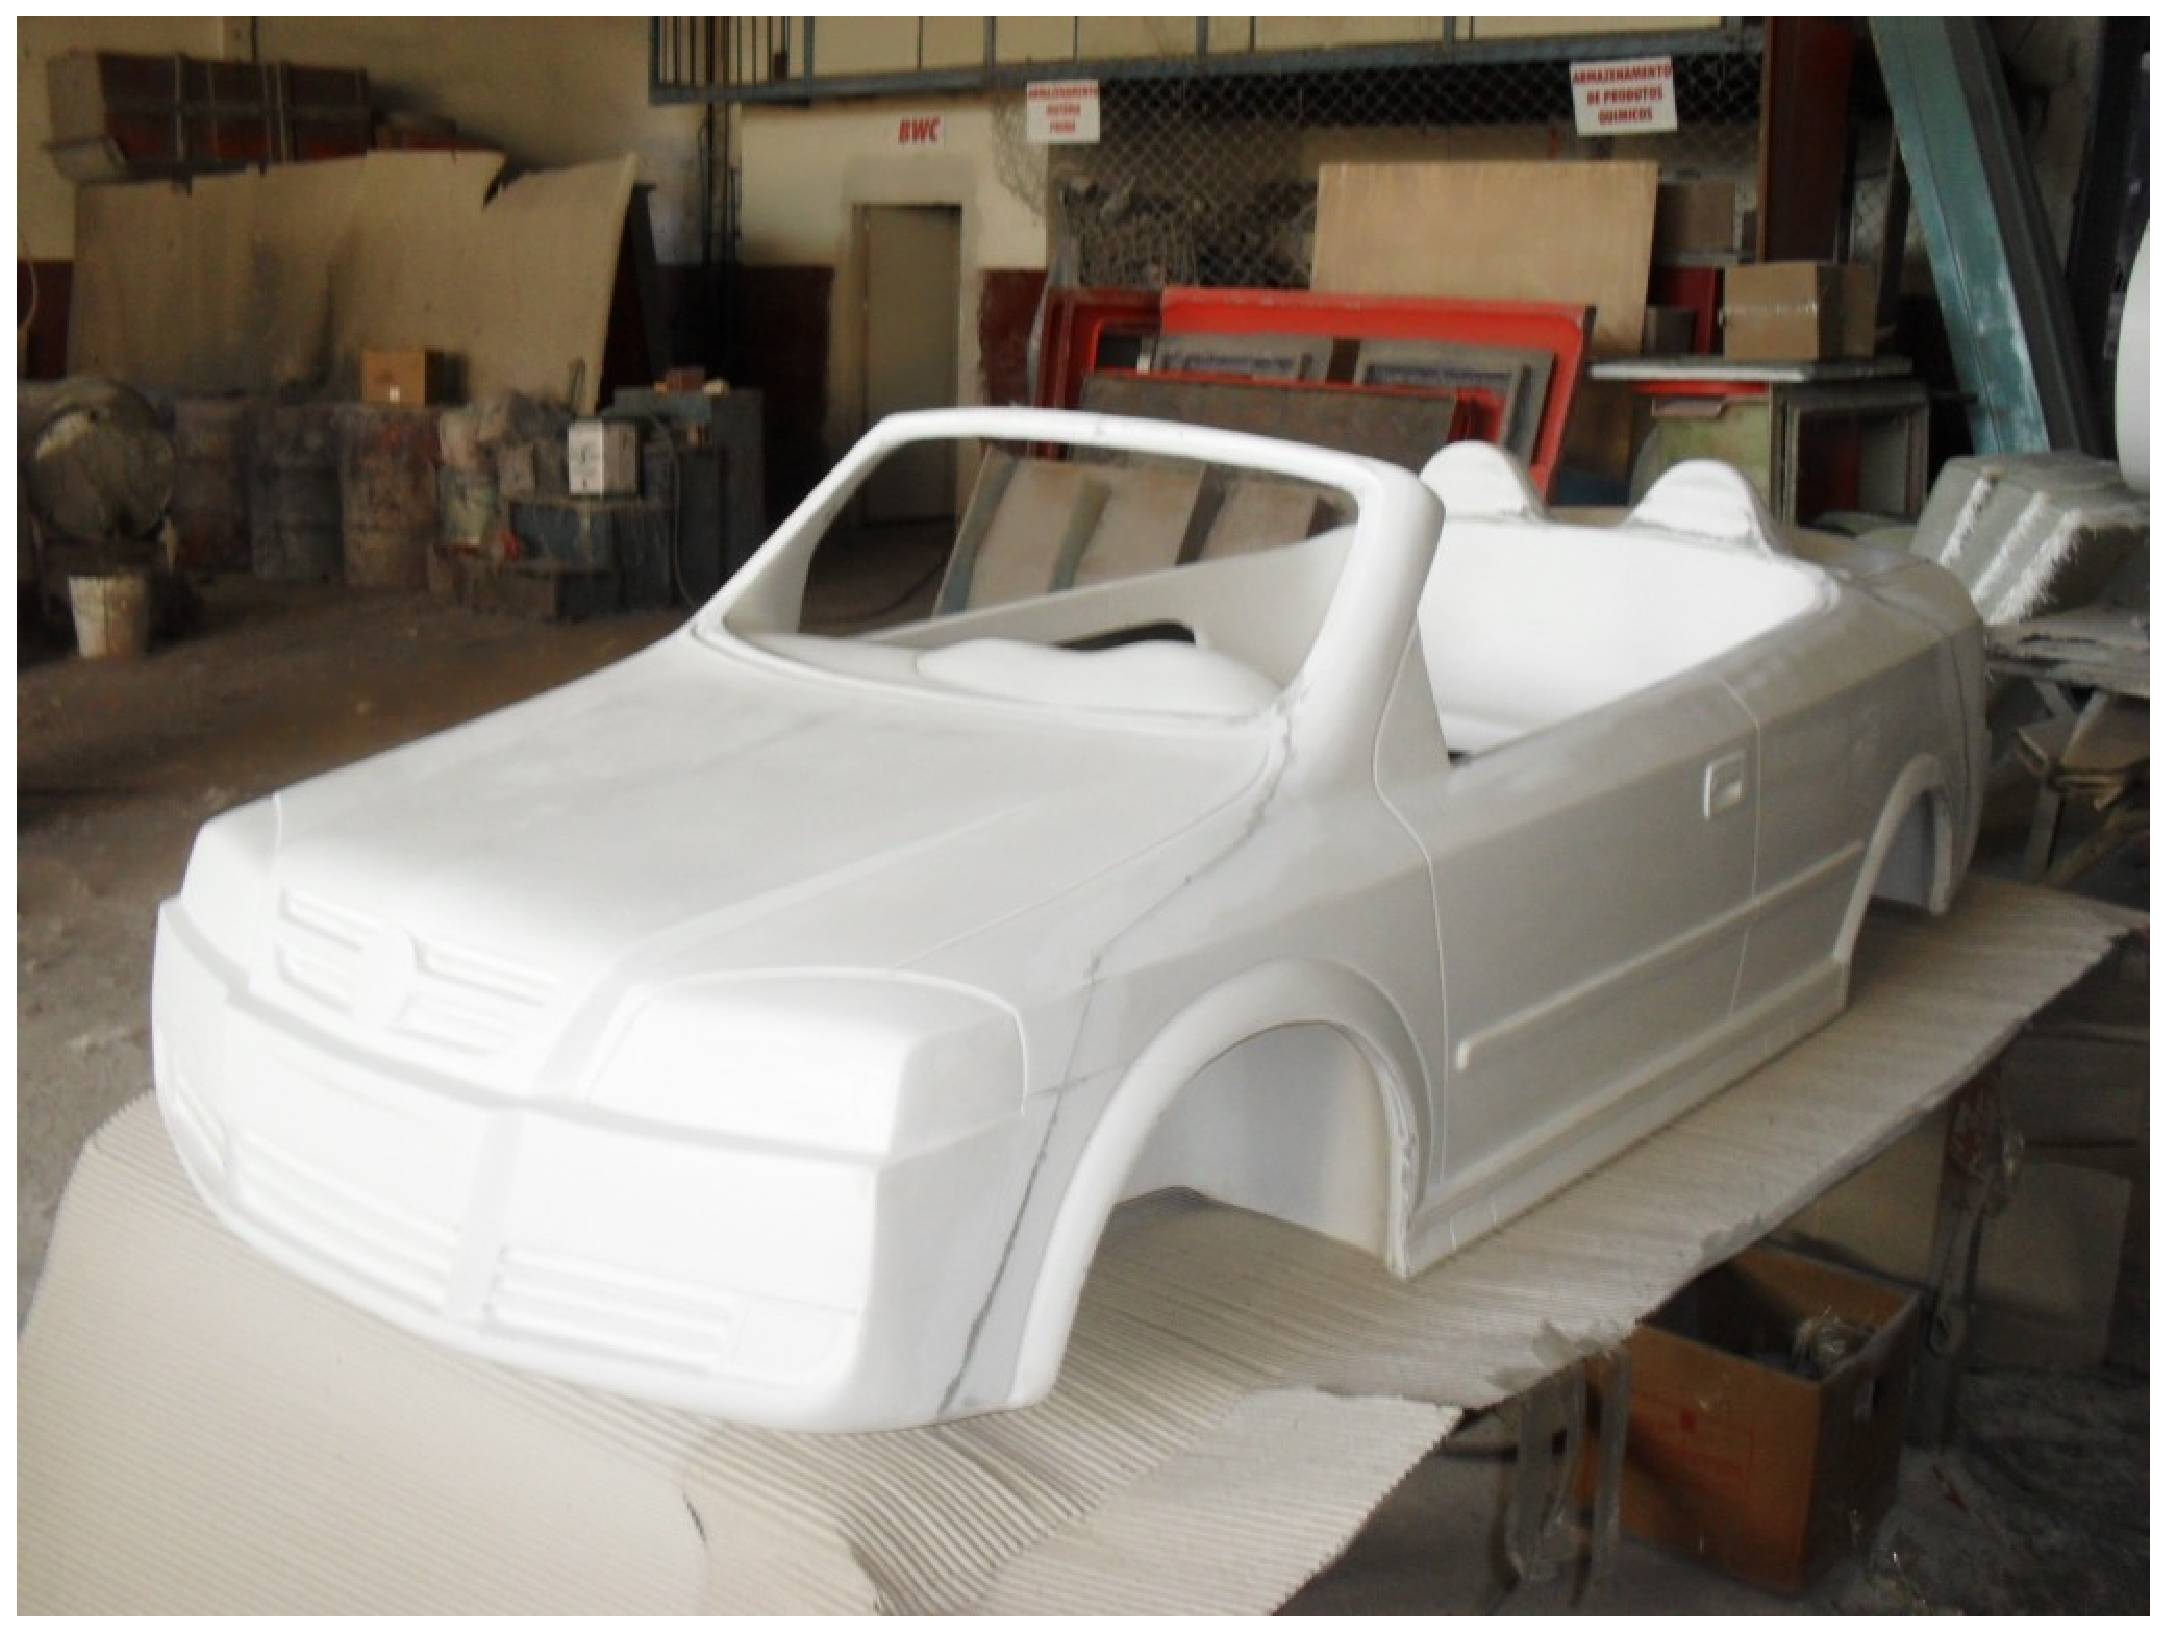
\includegraphics[width=2cm]{figuras/carenagem_fibra.eps}\\\hline
    			Tipo 2 & Plástico de fibra de carbono para impressora 3D & 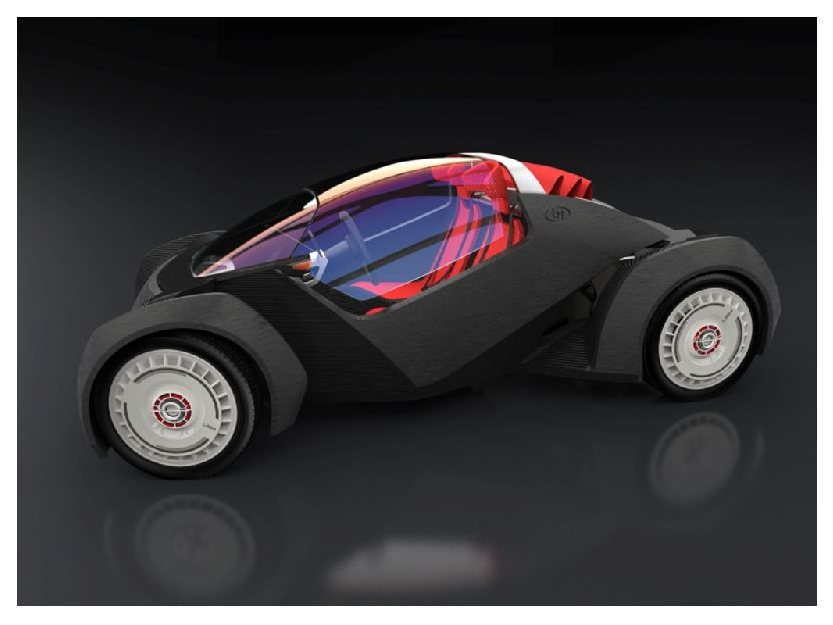
\includegraphics[width=2cm]{figuras/carenagem_plastico.eps}\\\hline
    		\end{tabular}
    	\end{center}
    \end{table}


    \newpage

  Ao comparar as características de cada material descrito acima, podemos chegar a conclusão que os melhores materiais que
  serão usados para a produção do veículo são:

  \begin{itemize}
    \item Roda + Pneu: a roda do tipo “off road”, pois a mesma é feita de material resistente e próprio para locomoção em estradas do tipo de terra. Já a roda de MBS possui o pneu de material inflável, logo o pneu pode furar durante o trajeto.
    \item Chassi: o chassi foi feito de aço metalon 20x20cm porque o aço proporciona alta resistência (1500 – 2000MPa), alto módulo de elasticidade, resistência à fadiga e tenacidade à fratura, possui baixo custo de fabricação e é fácil de ser manuseado.
    \item Eixo: o aço inox para este caso, se encaixa melhor, pois possui maior dureza do que seu comparativo disponível.
    \item Carenagem: a fibra de vidro é um dos materiais mais usados para esse tipo de aplicação, porque é de baixo custo e muito fácil de trabalhar. Já o plástico de fibra de carbono, tem um custo maior, precisa de uma impressora 3D para imprimir a peça e de um projeto feito em um software compatível com a  impressora. Ou seja, o plástico de carbono demanda custo e tempo para fabricar uma peça.
  \end{itemize}

\subsubsection{Testes Estruturais}

Os testes estruturais foram realizados utilizando o software de simulação Ansys. Foi utilizada para esse teste uma carga de 50kgf, que é consideravelmente maior do que a carga real que deverá ser suportada pela estrutura. As imagens a seguir ilustram o resultado das simulações. 

\begin{figure}[!htbp]
	\centering
	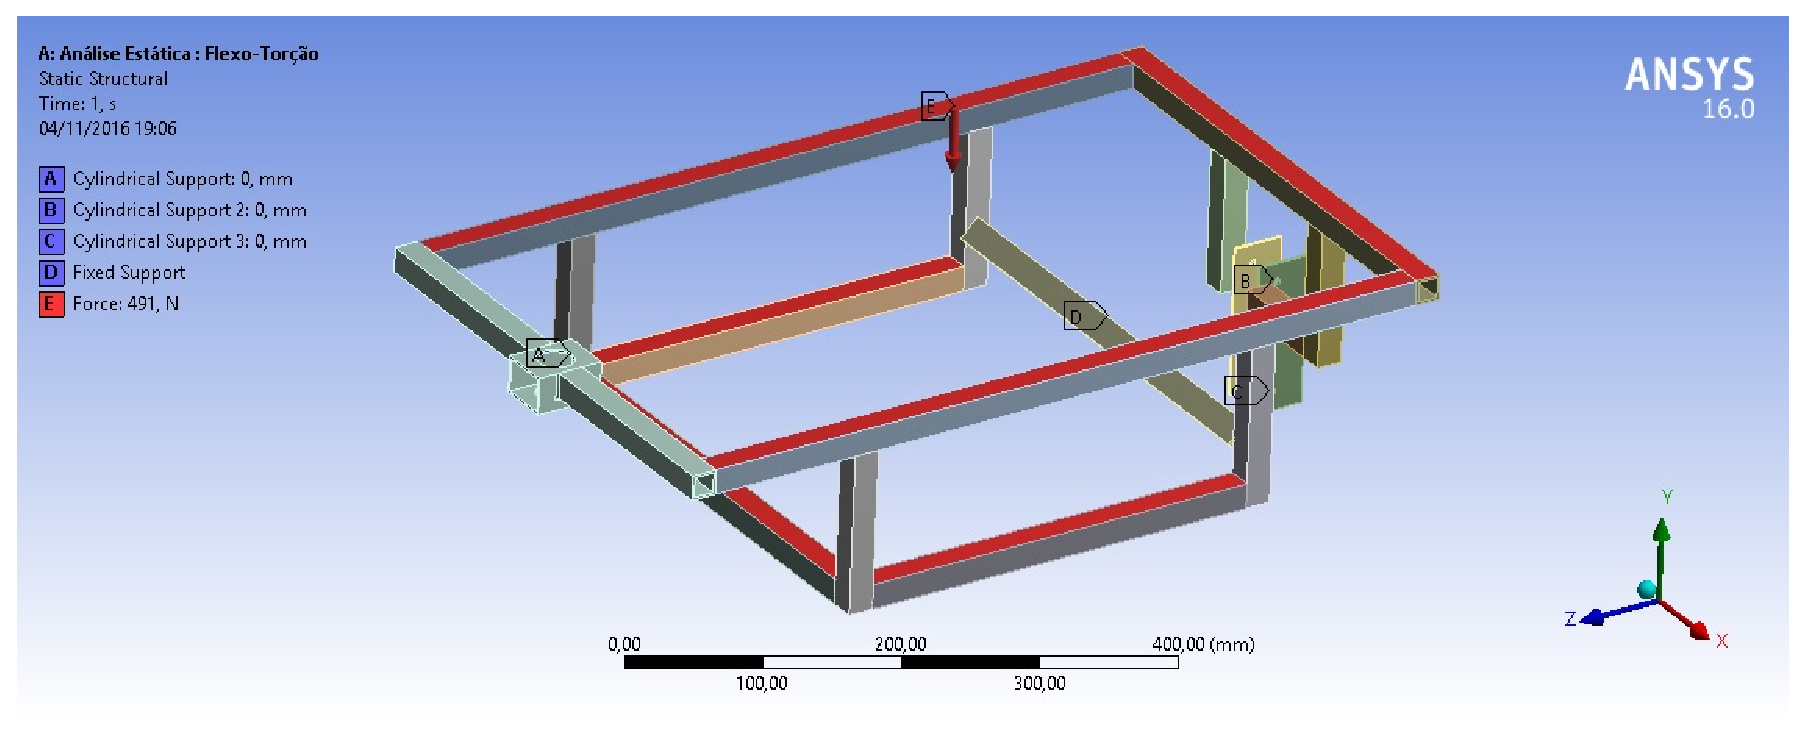
\includegraphics[width=.7\textwidth]{figuras/cond_contorno.eps}
	\caption{Condições de contorno da simulação}
\end{figure}

\begin{figure}[!htbp]
	\centering
	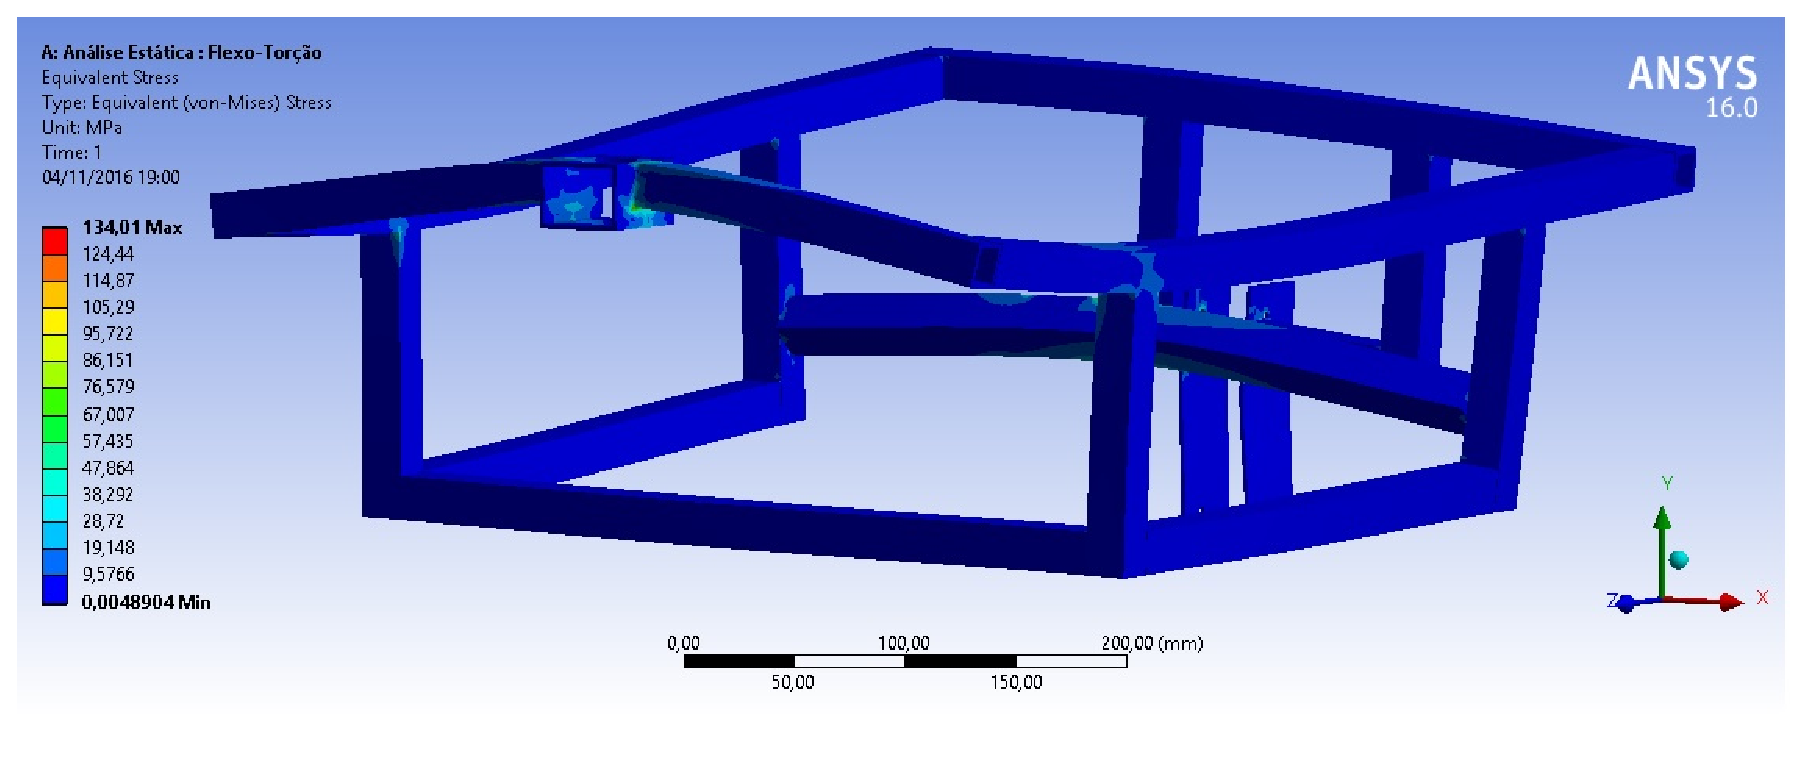
\includegraphics[width=.7\textwidth]{figuras/carga_distribuida1.eps}
	\caption{Carga distribuida da simulação}
\end{figure}

\begin{figure}[!htbp]
	\centering
	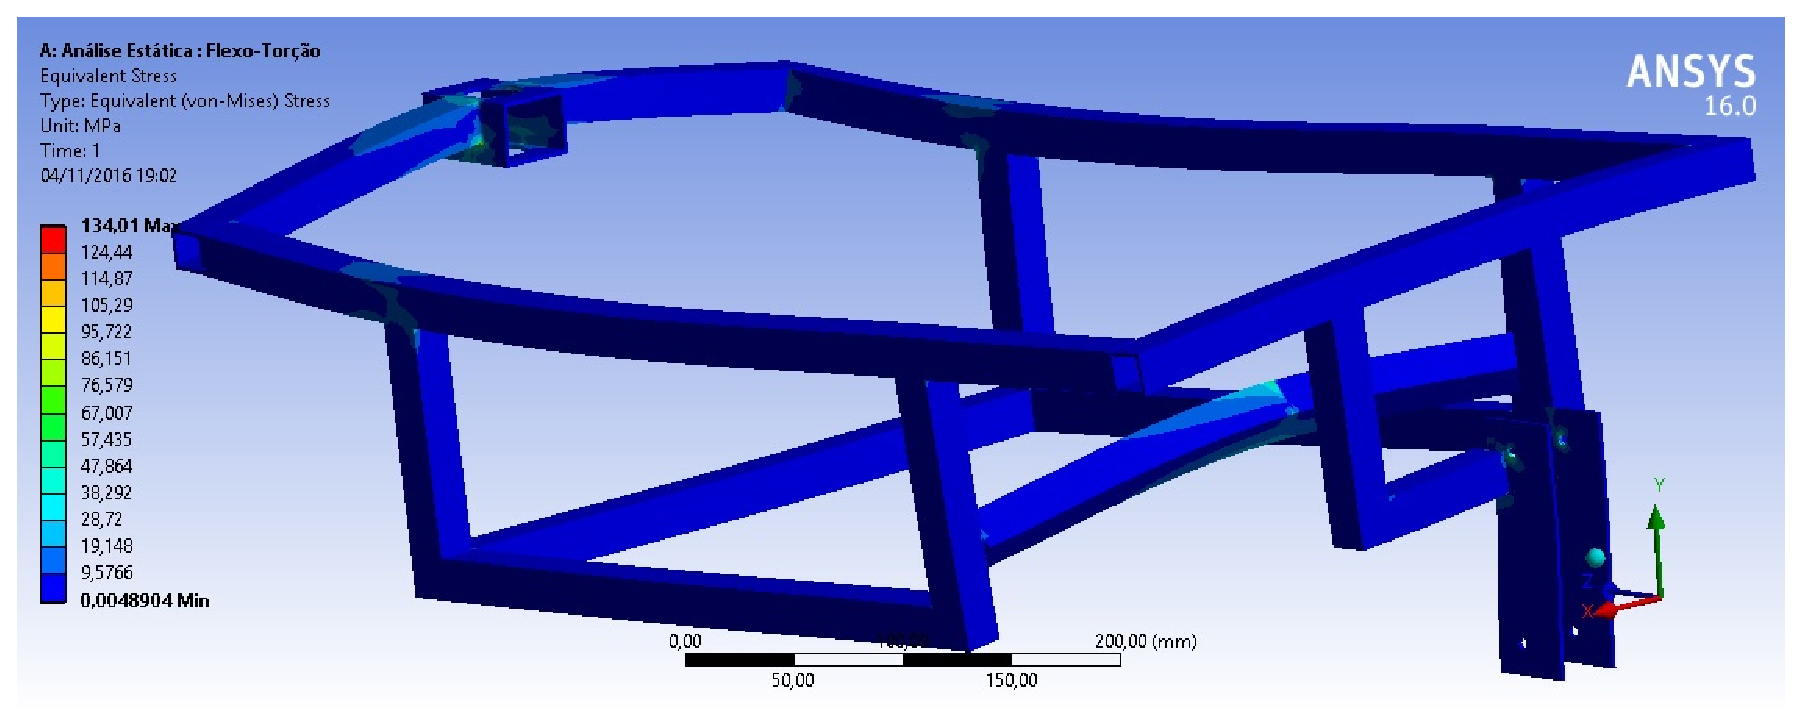
\includegraphics[width=.7\textwidth]{figuras/carga_distribuida2.eps}
	\caption{Carga distribuida da simulação}
\end{figure}

\begin{figure}[!htbp]
	\centering
	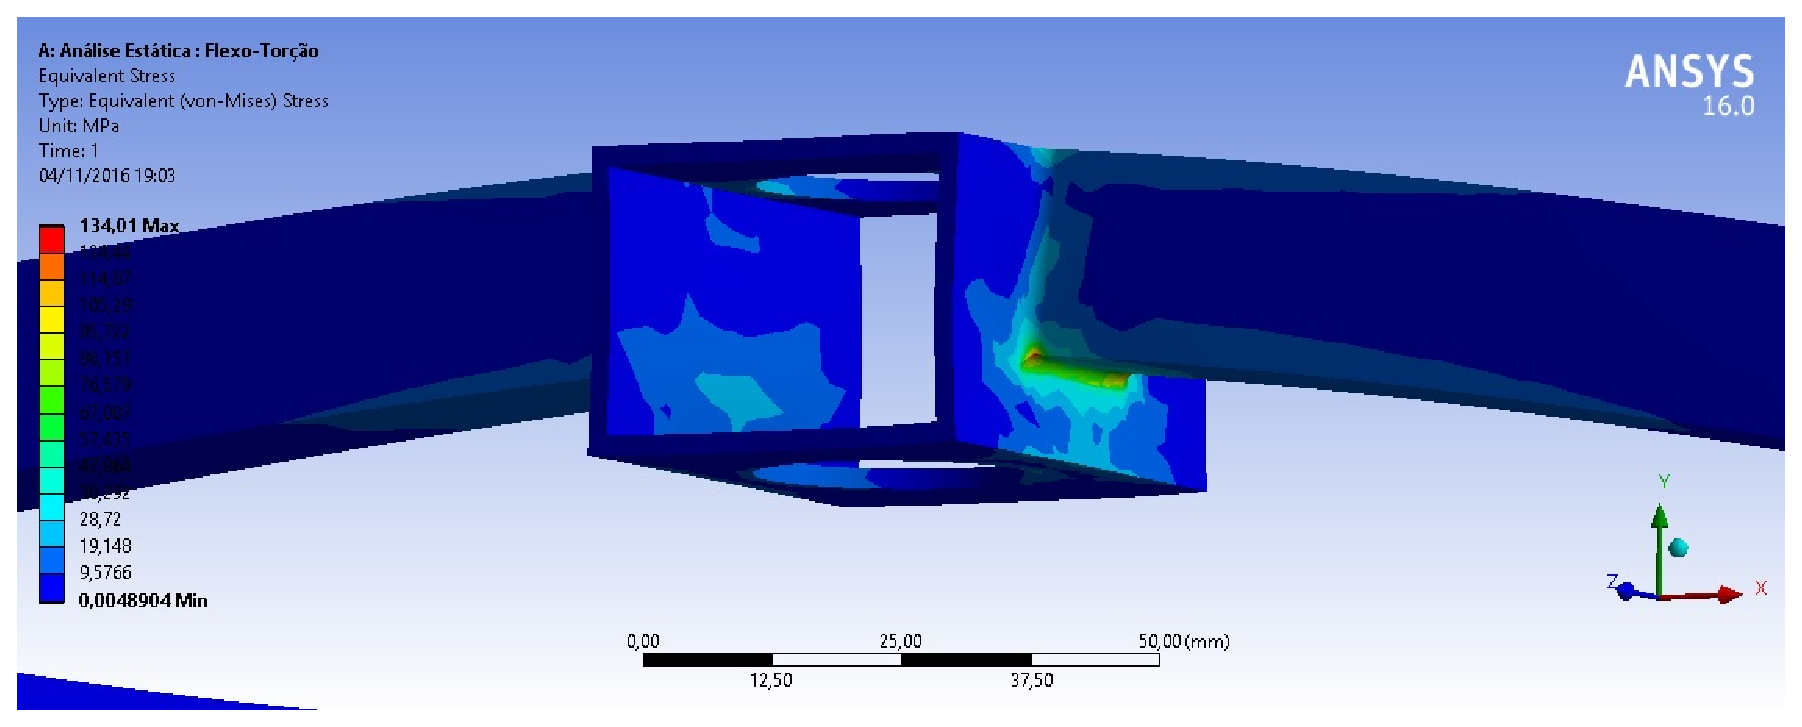
\includegraphics[width=.7\textwidth]{figuras/zoom_suporte.eps}
	\caption{Vista aproximada da falha no suporte de direção}
\end{figure}

Os resultados obtidos foram considerados satisfatórios e, a partir desse ponto, foi iniciado o processo de fabricação.

  \subsection{Sistema de Alimentação}

  \begin{itemize}
    \item Motores


 Para o projeto, os motores precisam apresentar um torque elevado e robustez devido ao ambiente em que será submetido, porém, não justifica o emprego de motores de precisão, como são os motores de passo. Portanto, a partir da análise das características dos motores existentes e considerando a satisfação dos requisitos do projeto, custos limitados e o tempo hábil para a construção e integração do rover em questão, os motores para tração escolhidos foram motores de corrente contínua.
 
 Sendo assim, determinou-se o uso de um motor de corrente contínua para atender à tração das rodas traseiras, as quais compartilham o mesmo eixo de transmissão através de uma caixa de redução. Essa escolha é justificada pela possibilidade de um terreno arenoso, altamente úmido e frequentemente com imperfeições e desníveis. A utilização deste motor garante que não haja atolamento e que o rover possa se locomover sem maiores dificuldades.
 
 Para o seu dimensionamento, foram considerados alguns parâmetros iniciais, como massa de 16 kg e velocidade de deslocamento de 0,12 m/s. Com isso, foi possível obter aproximadamente 6,7 N.m de torque e 40W de potência. Para atender a essa demanda, optou-se por utilizar um motor modelo Mabuchi GD – 558RC/LC 12 V. O qual possui 38 W e um torque máximo de 9,3 N.m.
 
 Para o sistema de direção do veiculo foi escolhido um motor de passo, representado na Figura \ref{fig:passo}. Este motor fornece movimentos precisos e são usados em aplicações em que o controle de ângulo de rotação, velocidade, posição e sincronismos são os requisitos. O ponto forte desse tipo de motor não é sua força (torque) e nem altas velocidades, mas é a capacidade de controle de forma acurada.  Portanto este dispositivo é amplamente usado em impressoras, scanners, robôs, câmaras de vídeo, brinquedos, automação industrial entre outros dispositivos eletrônicos \cite{brites}.
      
       \begin{figure}[!htbp]
       	\begin{center}
       		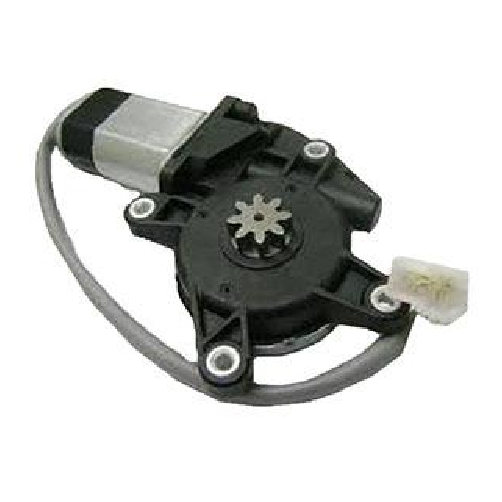
\includegraphics[keepaspectratio=true,scale=1]{figuras/mabuchi.eps}
       		\caption{Motor Mabuchi GD - 558RC/LC 12V}
       	\end{center}
       \end{figure}

         \begin{figure}[!htbp]
         	\begin{center}
         		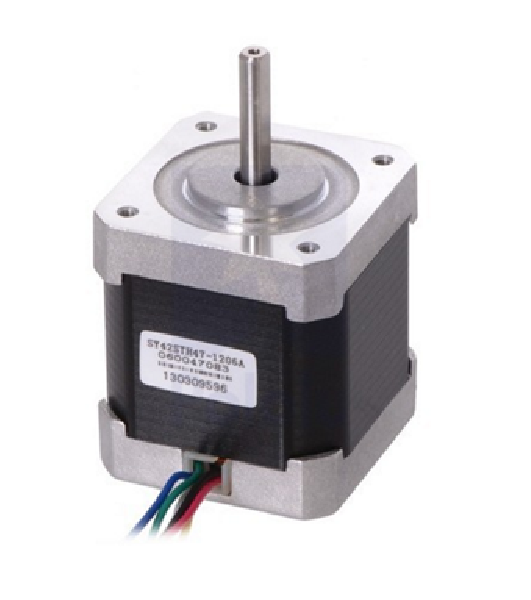
\includegraphics[keepaspectratio=true,scale=1]{figuras/passo.eps}
         		\caption{Motor de Passo - Modelo 22KM–0213G6V}
         		\label{fig:passo}
         	\end{center}
         \end{figure}     
            

     \item Bateria

    Algumas especificações devem ser observadas na seleção uma bateria, as mais importantes são a corrente e a
    tensão \cite{MAGALHAES}.

    Os cálculos de autonomia para as baterias não são triviais, necessitam de muitos parâmetros. Na literatura não
    há uma formulação exata para calcular esses valores. Portanto, são usadas diversas aproximações e parâmetros mais
    relevantes são determinados \cite{MEGGLIAR}.

    Três parâmetros principais que são apresentados: curva de descarga, a capacidade da bateria e a capacidade de
    descarga \cite{MEGGLIAR}.

    A curva de descarga representa o decaimento da tensão ao longo do consumo da capacidade nominal. O segundo parâmetro
    é a capacidade da bateria, o qual quantifica o tempo para que ocorra uma descarga total. Sua medida usual é Ah
    (Ampère x hora) \cite{MEGGLIAR}.

    A capacidade de descarga é quanto a bateria consegue fornecer sem que ocorra um superaquecimento, que poderia
    causar danos imensos a todo o projeto. Ela vem representada nas especificações pela letra C \cite{MEGGLIAR}.

    Alguns tipos de baterias poderiam ser selecionados para o projeto. A Bateria Íon- Lítio é o mais utilizado atualmente
    no mercado para aplicações em aparelhos eletrônicos, seu funcionamento consiste no uso de íons lítio presentes no
    eletrólito na forma sais dissolvidos em solventes não aquosos. Suas principais características são baixas taxas de auto
    descarga, longos ciclos de vida e segurança no manuseio \cite{castillo2002advances}.

    Em segundo, a bateria de polímero de lítio possui seus eletrólitos contidos em um polímero, diferentemente das baterias
    de íon-lítio, em que os eletrólitos estão contidos em solventes. As baterias de polímero de lítio são baterias de tecnologia
    ultrafinas. Isso é possível devido a sua maior densidade de energia quando comparada com as baterias de íon- lítio.

    Por fim, as baterias de chumbo-ácido são baterias comumente utilizadas em arranques e iluminação para automóveis,
    sistemas de tração para veículos e máquinas elétricas, além de serem utilizadas como fontes alternativas em nobreaks.
    Sua composição é chumbo, que está presente na forma sólida e ácido sulfúrico, em concentração que varia de 27\% a 37\% 
    \cite{pulsada2005juliano}. Se apresentam em dois formatos: seladas e não seladas, sendo que nesta segunda existe a necessidade de
    reposição de água. São baterias recarregáveis, pesadas, têm vida útil de até quatro anos e possuem custo-benefício satisfatório.

    Para o correto dimensionamento, levantou-se o consumo dos componentes do veículo, como pode ser visto na tabela \ref{tabeladimensionamento}.

     \begin{table}[!htbp]
     \centering
     \caption{Tabela de dimensionamento de consumo dos componentes}
     \label{tabeladimensionamento}
     \begin{tabular}{|p{4cm}|p{4cm}|p{4cm}|}
     \hline
     Componente          & Corrente Máxima & Tensão Nominal \\\hline
     Arduino             & 2 A             & 5 - 20 V       \\\hline
     Raspberry           & 2 A             & 5 V            \\\hline
     Driver              & 4 A cada        & 4-35 V         \\\hline
     Motor DC Tração     & 2 A         & 12 V           \\\hline
     Motor DC Perfuração & 2 A         & 12 V           \\\hline
     Motor de Passo          & 2 A             & 12 V            \\\hline
     \end{tabular}
     \end{table}

   Um ponto importante é observar que como os motores estarão conectados aos seus respectivos drivers de controle as correntes máximas são limitadas por eles. Como serão dois drivers de controle, a corrente máxima necessária será de 10 A - dois drivers mais a corrente do Arduino. Portanto, para 1 hora de operação em carga máxima, será necessário uma bateria de 10Ah. Tendo em vista que durante a operação do veículo, não haverá a utilização de todos os componentes em carga máxima ao mesmo tempo, a autonomia do veículo poderá vir a ser maior que o tempo estimado.
   
   Optou-se pelo modelo Get Power gp12-14, ela possui 12V e 7Ah. Para recarregar a bateria foi cogitado a utilização de um painel solar. Porém, a placa solar possui dimensões maiores que a estrutura do carro e um baixo ganho energético, em torno de apenas 3\%, o que não viabiliza a sua aplicação nesse projeto.
   

     \item Circuito Elétrico

     O diagrama unifilar apresentado na figura \ref{diagramaunifilar} representa as ligações a serem realizadas entre os componentes que serão utilizados.
     Após a bateria, será colocado um disjuntor monopolar (no ponto D) de 17,5 A de corrente alternada. Apesar de não ser de
     corrente contínua, ele satisfaz os requisitos de operação. Para o Arduino e para a Raspberry determinou-se dois fusíveis
     (F1 e F2) de 3 A.

     \begin{figure}[!htbp]
     \begin{center}
     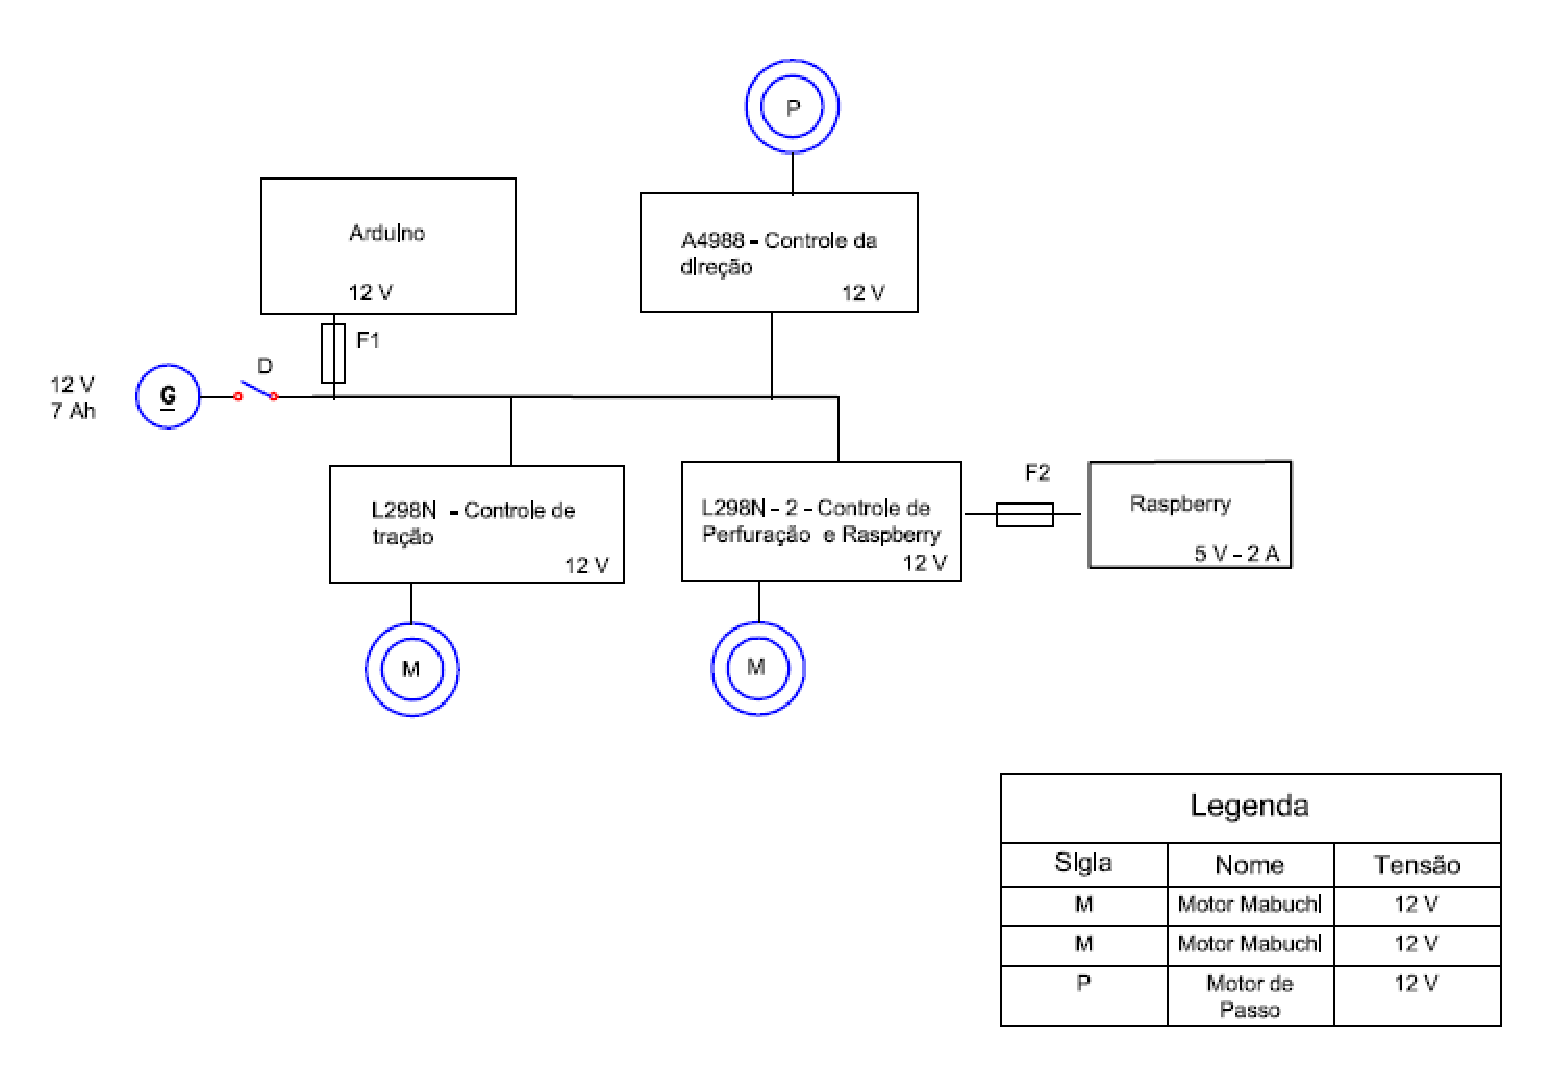
\includegraphics[keepaspectratio=true,scale=0.5]{figuras/unifilar.eps}
     \caption{\label{diagramaunifilar}Diagrama Unifilar dos Componentes}
     \end{center}
     \end{figure}

  \end{itemize}
